\begingroup 
\input{Back/IrieAPI/highlight}

\chapter{Platform Administration}\label{sec:administration}
% Please provide us with a data diagram of what is currently taking place and the roles and responsibilities of UCB and Caltrans specifically to each process.

% Please provide a list of all software/hardware that is used to run the current system.  If known, please provide a list of future hardware/software that will be required for BRACE2 as well.


\section{Hosting}
The software requirements are very flexible. The host server should be capable of supporting at least a standard Python 3.8 environment, but a newer version is recommended. The application has been successfully run on both cloud-hosted servers and a local server with a variety of operating systems and databases. All of these would be adequate options for Caltrans. On the \href{https://www.heroku.com}{Heroku} cloud hosting platform, with current demands, the application can easily be hosted for under \$20/month.

Both \emph{SQLite} and \emph{PostgreSQL} databases have been successfully used between various deployments, and any database supported by the Django framework should also be acceptable. 
Currently, Django officially supports \emph{PostgreSQL}, \emph{MariaDB}, \emph{MySQL}, \emph{Oracle}, and \emph{SQLite}{\footnote{More information on database support can be found in the Django database documentation page:  \url{https://docs.djangoproject.com/en/5.0/ref/databases/}.}}. 
Various deployment environments have been used successfully to host the platform. The Heroku stack that is currently hosting the instance at \url{https://structures.live} is summarized in Table \ref{tab:heroku-stack}. 
\begin{table}[h!]
    \centering
    \caption{Heroku stack currently employed in serving the \BRACE{} platform.}
    \begin{tabular}{ll}
    \toprule
        \textbf{Component} & \textbf{Product} \\ \hline
         Dyno & \texttt{eco} \\
         Datastore &  \texttt{postgresql-asymmetrical-28930} \\
         Gateway & \texttt{gunicorn } \\
    \bottomrule
    \end{tabular}
    \label{tab:heroku-stack}
\end{table}

\section{Installation}
The installation procedure is as follows:

\begin{enumerate}
\def\labelenumi{\arabic{enumi}.}
\item
  Create a virtual environment.

\item
  Install dependencies by executing the command:


\begin{Shaded}
\begin{Highlighting}[]
\NormalTok{ pip install }\AttributeTok{{-}r}\NormalTok{ requirements.txt}
\end{Highlighting}
\end{Shaded}

  \begin{quote}
  {[}Note{]} If you plan to run locally, comment out the following
  dependencies in \texttt{requirements.txt} by inserting a \texttt{\#}
  character.

  \begin{itemize}
  \tightlist
  \item
    psycopg2\textgreater=2.0,\textless3.0
  \item
    tcinter\textgreater=0.0.4
  \end{itemize}
  \end{quote}


\item
  Set up the database

\begin{Shaded}
\begin{Highlighting}[]
\ExtensionTok{python} \AttributeTok{{-}m}\NormalTok{ irie.init core.settings }
\end{Highlighting}
\end{Shaded}
\item 
  Create a superuser:

\begin{Shaded}
\begin{Highlighting}[]
\VariableTok{DEBUG}\OperatorTok{=}\NormalTok{True }\ExtensionTok{python}\NormalTok{ manage.py createsuperuser}
\end{Highlighting}
\end{Shaded}
\item
  Start the app

\begin{Shaded}
\begin{Highlighting}[]
\VariableTok{DEBUG}\OperatorTok{=}\NormalTok{True }\ExtensionTok{python}\NormalTok{ manage.py runserver}
\end{Highlighting}
\end{Shaded}

  The app should now be running at \texttt{http://127.0.0.1:8000/}.
\end{enumerate}


\section{Users and Groups}
Users of the application are divided into three \emph{groups}, based on their required privileges (see also \cref{fig:interaction,fig:database}):
\begin{description}
    \item[Group 1] consists of agents (currently, only California Geological Survey ``CGS'' and its California Strong Motion Instrumentation Program ``\href{https://www.conservation.ca.gov/cgs/smi/program}{CSMIP}'', which hosts and manages the Center for Engineering Strong Motion Data ``\href{https://www.strongmotioncenter.org/}{CESMD}'') that provide ground motion data in real-time. This is the only group that will most likely need access from outside of the host's local network. This user group makes \texttt{POST} requests over a secured API (\cref{ch:event-api}) that is provided by the \texttt{brace2.events} sub-application. These posts contain a ground motion archive file that must be stored temporarily on the disk while the \emph{predictors} are executed. 
    Any data from these files that is needed for long-term operations on the platform is parsed out and stored as an entry in the \texttt{Event} database table. 
    %
    \item[Group 2] consists of users (likely engineers within the host's local network, i.e., Caltrans) that will be granted privileges to configure inventory predictors. These users will interact with the platform over a standard
    web browser by accessing HTML{\footnote{HyperText Markup Language (HTML) is the standard markup language for documents designed to be displayed in a web browser.}} pages that are served by the \texttt{brace2.inventory} and \texttt{brace2.predictors} sub-applications. These actions may result in insertions and deletions
    in the \texttt{Asset} and \texttt{Predictor} database tables.
    %
    \item[Group 3] consists of users with the same \emph{read} privileges as \textbf{Group 2}, but no \emph{write} privileges. The interactions from this group should not result in any changes to the database.
\end{description}
\begin{figure}[h!]
    \centering
    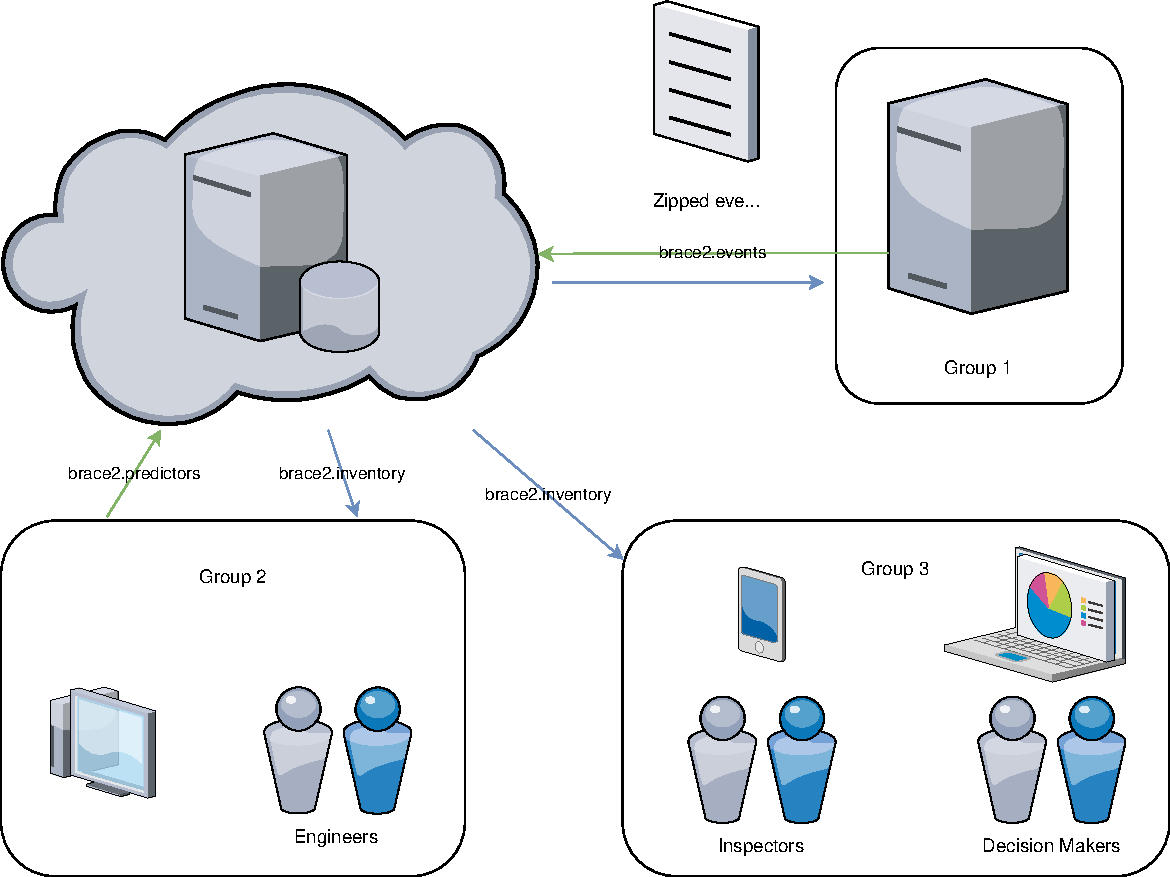
\includegraphics[width=\linewidth]{Back/IrieAdmin/Figures//BRACE2 Overview.pdf}
    \caption{\BRACE{} platform user access.}
    \label{fig:interaction}
\end{figure}
\begin{figure}[h!]
    \centering
    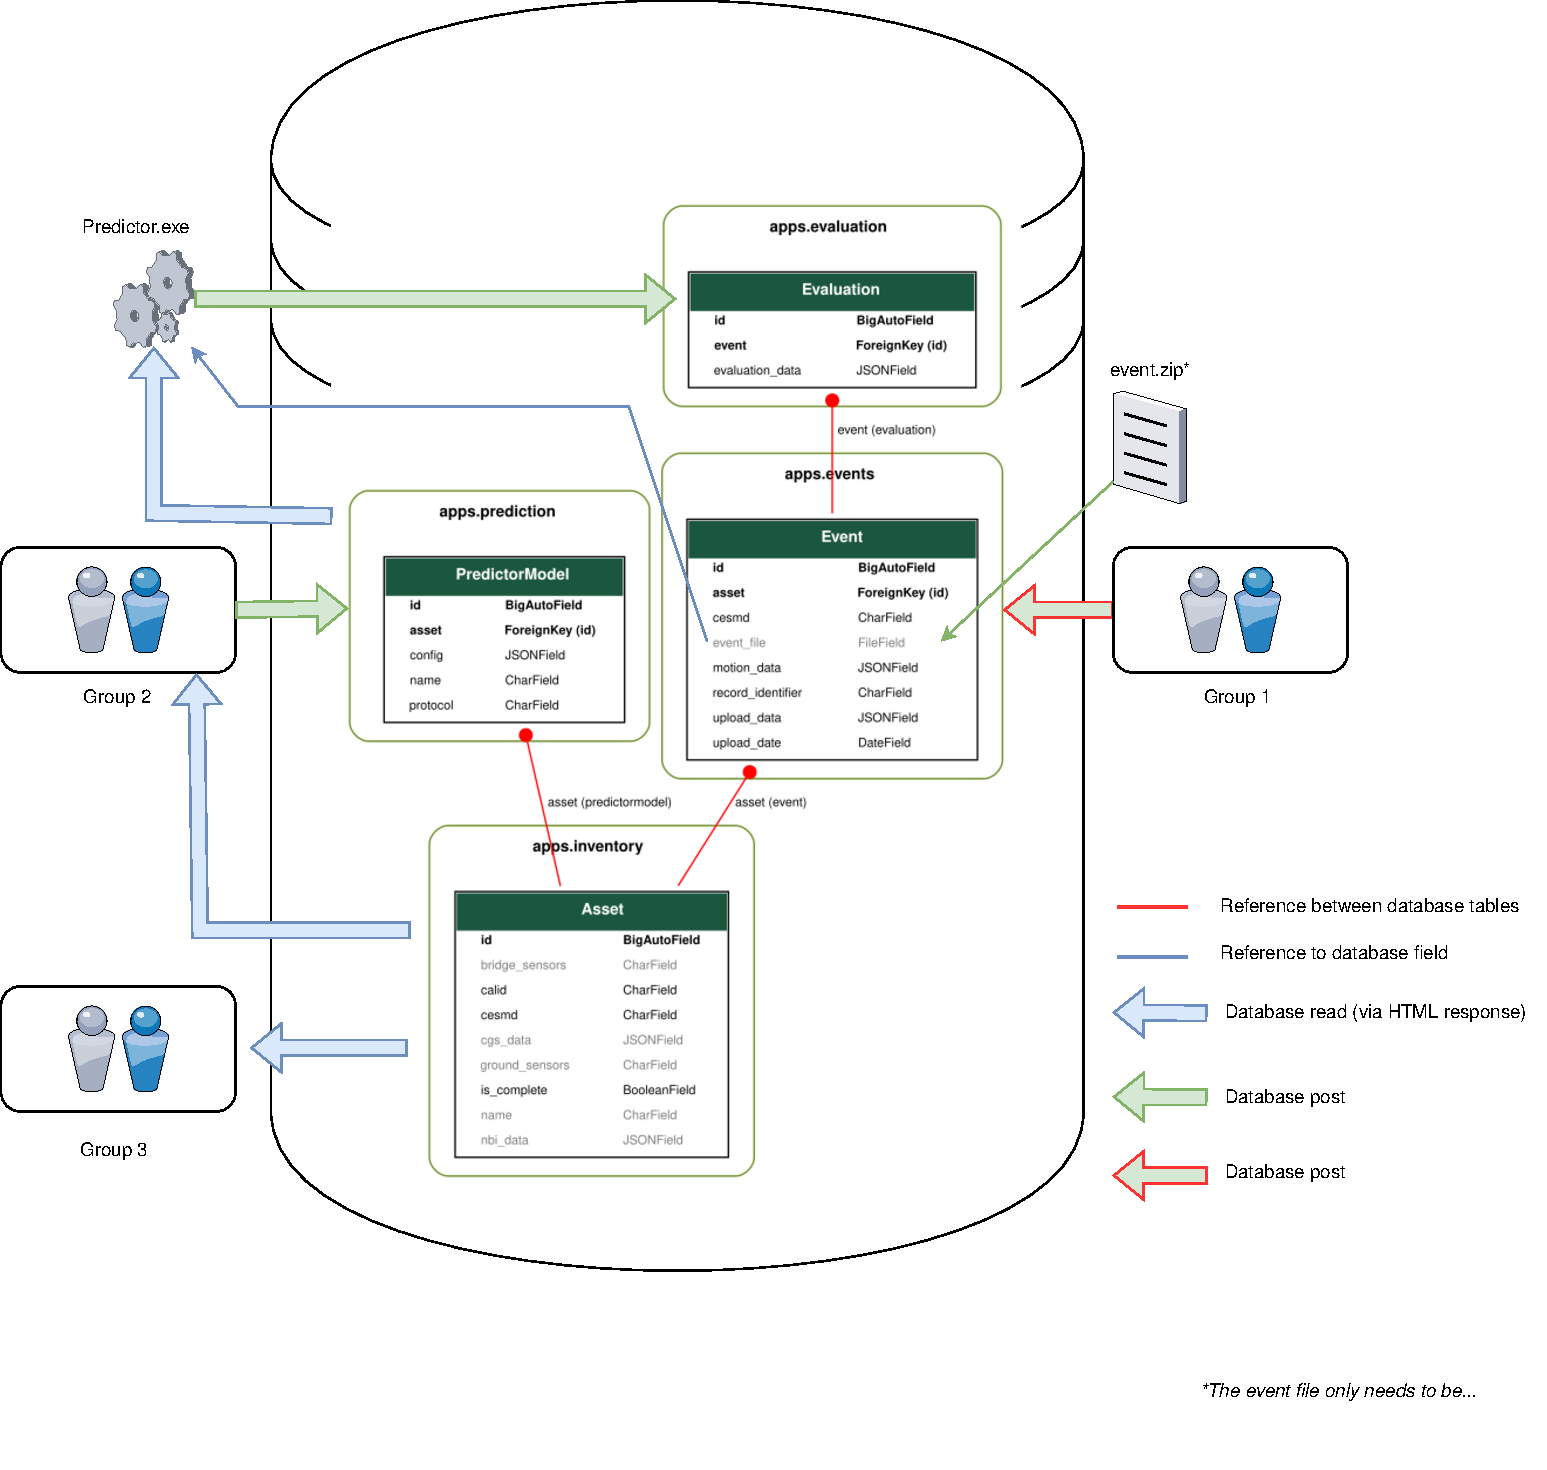
\includegraphics[width=\linewidth,trim={0 2cm 0 0},clip]{Back/IrieAdmin/Figures//BRACE2 Database.pdf}
    \caption{\BRACE{} platform database implementation details.}
    \label{fig:database}
\end{figure}

\section{Initializing the Pilot Models}

Once the platform is deployed, it can be populated further by performing the following steps:
\begin{description}
\item[0) Initialize environment:] Make sure that the proper Python environment
is activated in the working shell and the current working directory
is the root of the \texttt{HealthMonitoringPlatform} repository.

\item[1) Install initialization dependencies:]
The initialization process requires a few additional dependencies. These
can be installed by running the following command:
%
\begin{Shaded}
\begin{Highlighting}[]
\ExtensionTok{python} \AttributeTok{{-}m}\NormalTok{ pip install }\AttributeTok{{-}Ur}\NormalTok{ init/requirements.txt}
\end{Highlighting}
\end{Shaded}

\item[{2) Configure partial twins} (optional):]
Assets and predictors will be configured from the files \texttt{init/bridges.py} and \texttt{init/calid.py}. These can be modified or extended before proceeding.

\item[3) Download CGS data:]
The following script will execute the file \texttt{init/bridges.py} and
pull CGS metadata for the bridges listed there:
%
\begin{Shaded}
\begin{Highlighting}[]
\ExtensionTok{python}\NormalTok{ init/getCGSData.py  }\OperatorTok{\textgreater{}}\NormalTok{ data/cgs\_data.json}
\end{Highlighting}
\end{Shaded}

\item[4) Create assets (bridges):]
Run the following command to create an \texttt{Asset} in the database for
each of the bridges listed in \texttt{bridges.py}:
%
\begin{Shaded}
\begin{Highlighting}[]
\ExtensionTok{python}\NormalTok{ manage.py shell }\OperatorTok{\textless{}}\NormalTok{ init/init\_assets.py}
\end{Highlighting}
\end{Shaded}

\item[5) Create predictors:]
Run the following command to create a \texttt{PredictorModel} in the
database for each of the predictors listed in \texttt{bridges.py}:
\begin{Shaded}
\begin{Highlighting}[]
\ExtensionTok{python}\NormalTok{ manage.py shell }\OperatorTok{\textless{}}\NormalTok{ init/init\_predictors.py}
\end{Highlighting}
\end{Shaded}
\end{description}

%The credentials needed to access the platform can be obtained by contacting the authors of this report or the Office of Earthquake Engineering Analysis \& Research (OEEAR), Caltrans.

% Once this setup is completed, users can be created with credentials in the standard manner using the Django admin page. For more information, refer to the Django documentation: \url{https://docs.djangoproject.com/en/5.0/ref/}.

\endgroup